%%%%%%%%%%%%%%%%%%%%%%%%%%%%%%%%%%%%%%%%%%%%%%%%%%%%%%%%%%%%%%%%%%%%
%% I, the copyright holder of this work, release this work into the
%% public domain. This applies worldwide. In some countries this may
%% not be legally possible; if so: I grant anyone the right to use
%% this work for any purpose, without any conditions, unless such
%% conditions are required by law.
%%%%%%%%%%%%%%%%%%%%%%%%%%%%%%%%%%%%%%%%%%%%%%%%%%%%%%%%%%%%%%%%%%%%

\documentclass{beamer}
\usetheme[faculty=ped,basePath=../fibeamer,logo=../fibeamer/logo/mu/Logo-UC-3.png]{fibeamer}
\graphicspath{{../resources/}}

\usepackage{algorithm}
\usepackage{algpseudocode}

\usetheme[faculty=ped]{fibeamer}
\usepackage[utf8]{inputenc}
\usepackage[
  main=english, %% By using `czech` or `slovak` as the main locale
                %% instead of `english`, you can typeset the
                %% presentation in either Czech or Slovak,
                %% respectively.
  czech, slovak %% The additional keys allow foreign texts to be
]{babel}        %% typeset as follows:
%%
%%   \begin{otherlanguage}{czech}   ... \end{otherlanguage}
%%   \begin{otherlanguage}{slovak}  ... \end{otherlanguage}
%%
%% These macros specify information about the presentation
\title{String} %% that will be typeset on the
\subtitle{Semestre II-2026} %% title page.
\author{Profesora: Andreina Cota Vidaurre}
%% These additional packages are used within the document:
\usepackage{ragged2e}  % `\justifying` text
\usepackage{booktabs}  % Tables
\usepackage{tabularx}
\usepackage{tikz}      % Diagrams
\usetikzlibrary{calc, shapes, backgrounds}
\usetikzlibrary{positioning, arrows.meta, shadows.blur, shapes.geometric}
\usepackage{amsmath, amssymb}
\usepackage{url}       % `\url`s
\usepackage{listings}  % Code listings
\usepackage{graphicx}
\usepackage{amsmath}
\usepackage[T1]{fontenc}
\usepackage{xcolor}
\usepackage{minted}
% \usepackage{adjustbox}


% Definicion de pseudocodigo en espaniol
\lstdefinelanguage{PseudocodigoES}{
    morekeywords={INICIO,FIN,PARA,HACER,SI,ENTONCES,FIN_SI,FIN_PARA,IMPRIMIR},
    sensitive=true,
    morecomment=[l]{//},
    morestring=[b]"
}

% Definicion de pseudocodigo en ingles
\lstdefinelanguage{PseudocodeEN}{
    morekeywords={BEGIN,END,FOR,DO,IF,THEN,END_IF,END_FOR,PRINT},
    sensitive=true,
    morecomment=[l]{//},
    morestring=[b]"
}

\lstset{
    basicstyle=\ttfamily\small,
    keywordstyle=\bfseries,
    columns=fullflexible,
    keepspaces=true,
    showstringspaces=false,
    frame=single,
    xleftmargin=0em,
    framexleftmargin=0em,
    framesep=2pt,
    gobble=4,
    resetmargins=true,
    aboveskip=0pt,
    belowskip=0pt
}

\lstdefinestyle{pythonstyle}{
    language=Python,
    basicstyle=\ttfamily\small,
    keywordstyle=\bfseries,
    commentstyle=\itshape,
    stringstyle=\ttfamily,
    showstringspaces=false,
    columns=fullflexible,
    keepspaces=true,
    frame=single,
    breaklines=true,
    xleftmargin=0em,
    framexleftmargin=0em,
    framesep=2pt,
    aboveskip=0pt,
    belowskip=0pt,
    gobble=4,
    resetmargins=true,
    emph={print,input,int,float,str,bool,len,range},
    emphstyle=\bfseries
}

\lstset{style=pythonstyle}

% Estilos del diagrama
\tikzstyle{iniciofin} = [
    ellipse,
    minimum width=2.5cm,
    minimum height=1cm,
    text centered,
    draw=black,
    fill=blue!25
]

\tikzstyle{proceso} = [
    rectangle,
    rounded corners,
    minimum width=3cm,
    minimum height=1cm,
    text centered,
    draw=black,
    fill=cyan!20
]

\tikzstyle{decision} = [
    diamond,
    aspect=2,
    text centered,
    draw=black,
    fill=yellow!35
]

\tikzstyle{flecha} = [
    thick,
    ->,
    >=Stealth
]

% \definecolor{green_python}{HTML}{52A736}

% \newcolumntype{Y}{>{\raggedright\arraybackslash}X}

\frenchspacing
\begin{document}
  \shorthandoff{-}
  \frame[c]{\maketitle}

% \begin{darkframes}

    \begin{frame}{Contenido}
        \begin{itemize}
            \item String
            \item Métodos y funciones
            \item String y ADN
            \item Propiedad del string
            \item Características del string
        \end{itemize}
    \end{frame}

    \begin{frame}{¿Qué es un string?}
        \begin{itemize}
            \item Un string es texto almacenado en memoria que el programa puede manipular
            \item Es uno de los tipos de datos más fundamentales en programación
            \item Casi todo lo que interactúa con las personas involucra texto
            \item En la práctica, los strings se usan en:
            \begin{itemize}
                \item Interfaces de usuario: Cualquier mensaje que se muestre al usuario
                \item Archivos y datos: Lectura de un archivo de texto o página web
                \item Comunicación con sistemas: Las URLs, correos electrónicos
                \item Validación de datos: Verificar que un RUT tiene el formato correcto
            \end{itemize}
        \end{itemize}
    \end{frame}

    \begin{frame}{¿Qué es un string?}
        \begin{itemize}
            \item Un \textbf{string} o cadena de texto es una secuencia ordenada de caracteres en Python
            \item En Python, un string es inmutable. Es decir, no se puede modificar una vez creado
            \item Puede contener letras, números, espacios, símbolos o cualquier carácter Unicode
            \item Se crea encerrando texto entre comillas simples '...', dobles "...", o triples '''...''' / """...""" para texto multilínea
            \item Cada carácter ocupa una posición llamada \textbf{índice}, comenzando desde 0 por la izquierda o desde -1 por la derecha
        \end{itemize}
        \centering

        \Large
        \begin{tabular}{c c c c c c}
        \textcolor{blue}{0} & \textcolor{blue}{1} & \textcolor{blue}{2} & \textcolor{blue}{3} & \textcolor{blue}{4} & \textcolor{blue}{5} \\
        P & y & t & h & o & n \\
        \textcolor{magenta}{-6} & \textcolor{magenta}{-5} & \textcolor{magenta}{-4} & \textcolor{magenta}{-3} & \textcolor{magenta}{-2} & \textcolor{magenta}{-1}
        \end{tabular}
    \end{frame}

    \begin{frame}[fragile,t]{String}
        \begin{minted}[xleftmargin=-2cm, frame=leftline, fontsize=\small]{python}
            texto = "Python"
            tipo  = type(texto)     # <class 'str'>
            
            # Tres formas de crear strings
            a = 'comillas simples'
            b = "comillas dobles"
            c = """texto
            multilínea"""
        \end{minted}
    \end{frame}    

    \begin{frame}[fragile,t]{Métodos y funciones}
        Siendo \mintinline{python}{x} una variable de tipo \mintinline{python}{str}
        \begin{itemize}
            \item \mintinline{python}{len(x)}: Devuelve el número de caracteres del string.
            \begin{minted}[xleftmargin=-2cm, frame=leftline, fontsize=\small]{python}   
            texto = "Python"
            len(texto)        # 6
            \end{minted}
            \item \mintinline{python}{x[i]}: Accede al carácter en la posición \textbf{i}. Los índices negativos cuentan desde el final.
            \begin{minted}[xleftmargin=-2cm, frame=leftline, fontsize=\small]{python}
            texto = "Python"
            texto[2]        # t
            \end{minted}
            \item \mintinline{python}{x[a:b]}: Extrae una subcadena desde el índice a (incluido) hasta b (excluido).
            \begin{minted}[xleftmargin=-2cm, frame=leftline, fontsize=\small]{python}
            texto = "Python"
            texto[0:3]          # Pyt
            \end{minted}
        \end{itemize}
    \end{frame}

    \begin{frame}[fragile,t]{Métodos y funciones}
        Siendo \mintinline{python}{x} una variable de tipo \mintinline{python}{str}
        \begin{itemize}
            \item \mintinline{python}{x in str}: Verifica si una subcadena existe dentro del string. Devuelve \mintinline{python}{True o False}
            \begin{minted}[xleftmargin=-2cm, frame=leftline, fontsize=\small]{python}
            "th" in "Python"        # True
            \end{minted}
            \item \mintinline{python}{upper()}: Devuelve una copia del string con todos los caracteres en mayúscula.
            \begin{minted}[xleftmargin=-2cm, frame=leftline, fontsize=\small]{python}
            "python".upper()        # PYTHON
            \end{minted}
            \item \mintinline{python}{lower()}: Devuelve una copia del string con todos los caracteres en minúscula.
            \begin{minted}[xleftmargin=-2cm, frame=leftline, fontsize=\small]{python}
            "PYTHON".lower()          # python
            \end{minted}
        \end{itemize}
    \end{frame}

    \begin{frame}[fragile,t]{Métodos y funciones}
        \begin{itemize}
            \item \mintinline{python}{isupper()}: Retorna \mintinline{python}{True} si todos los caracteres alfabéticos están en mayúscula.
            \begin{minted}[xleftmargin=-2cm, frame=leftline, fontsize=\small]{python}
            "PYTHON".isupper()          # True
            \end{minted}
            \item \mintinline{python}{islower()}: Retorna \mintinline{python}{True} si todos los caracteres alfabéticos están en minúscula.
            \begin{minted}[xleftmargin=-2cm, frame=leftline, fontsize=\small]{python}
            "python".islower()          # True
            \end{minted}
            \item \mintinline{python}{isdigit()}: Retorna True si todos los caracteres son dígitos (0-9).
            \begin{minted}[xleftmargin=-2cm, frame=leftline, fontsize=\small]{python}
            "2026".isdigit()          # True
            \end{minted}
            \item \mintinline{python}{isalpha()}: Retorna \mintinline{python}{True} si todos los caracteres son letras (a-z, A-Z).
            \begin{minted}[xleftmargin=-2cm, frame=leftline, fontsize=\small]{python}
            "Python".isalpha()          # True
            "Python3".isalpha()         # False
            \end{minted}
        \end{itemize}
    \end{frame}

    \begin{frame}[fragile,t]{Métodos y funciones}
        \begin{itemize}
            \item \mintinline{python}{isalnum()}: Retorna \mintinline{python}{True} si todos los caracteres son letras (a-z, A-Z) o números.
            \begin{minted}[xleftmargin=-2cm, frame=leftline, fontsize=\small]{python}
            "Python3".isalnum()          # True
            \end{minted}
            \item \mintinline{python}{strip()}: Elimina espacios (u otros caracteres) al inicio y al final del string.
            \begin{minted}[xleftmargin=-2cm, frame=leftline, fontsize=\small]{python}
            "       python      ".strip()          # python
            \end{minted}
            \item \mintinline{python}{find()}: Devuelve el índice de la primera aparición de la subcadena. Retorna -1 si no se encuentra.
                \begin{minted}[xleftmargin=-2cm, frame=leftline, fontsize=\small]{python}
            texto = "programacion"
            texto.find("gra")           # 3
            \end{minted}
        \end{itemize}
    \end{frame}

    \begin{frame}[fragile,t]{Métodos y funciones}
        \begin{itemize}
            \item \mintinline{python}{find(subcadena, inicio, fin)}: Devuelve el índice de la primera aparición de la subcadena entre 
            los índices inicio y fin.
            \begin{minted}[xleftmargin=-2cm, frame=leftline, fontsize=\small]{python}
            texto = "programacion"
            texto.find("gra", 3, 10)           # 3
            texto.find("gra", 11, 20)           # -1
            \end{minted}
            \item \mintinline{python}{count()}: Cuenta cuántas veces aparece la subcadena en el string.
            \begin{minted}[xleftmargin=-2cm, frame=leftline, fontsize=\small]{python}
            "programacion".count("a")       # 2
            \end{minted}
            \item \mintinline{python}{count(subcadena, inicio, fin)}: Cuenta cuántas veces aparece la subcadena entre los índices 
            inicio y fin.
            \begin{minted}[xleftmargin=-2cm, frame=leftline, fontsize=\small]{python}
            texto = "programacion"
            texto.count("a", 3, 10)           # 2
            texto.count("a", 11, 20)           # 0
            \end{minted}
        \end{itemize}
    \end{frame}

    \begin{frame}[fragile,t]{Métodos y funciones}
        \begin{itemize}
            \item \mintinline{python}{replace()}: Reemplaza todas las apariciones de una subcadena por otra.
            \begin{minted}[xleftmargin=-2cm, frame=leftline, fontsize=\small]{python}
            texto = "Hola estudiante"
            texto.replace("estudiante", "profesor")
            \end{minted}
            \item \mintinline{python}{split()}: Divide el string en una lista de subcadenas usando el separador indicado.
            \begin{minted}[xleftmargin=-2cm, frame=leftline, fontsize=\small]{python}
            "Universidad,Catolica".split(",")         # ['Universidad', 'Catolica']
            \end{minted}
            \item \mintinline{python}{join()}: Une los elementos de un iterable en un string insertando el separador entre ellos.
            \begin{minted}[xleftmargin=-2cm, frame=leftline, fontsize=\small]{python}
            "-".join("Hola")        # H-o-l-a
            \end{minted}
        \end{itemize}
    \end{frame}

    \begin{frame}[fragile,t]{Métodos y funciones}
        \begin{itemize}
            \item \mintinline{python}{startswith()}: Retorna \mintinline{python}{True} si el string empieza con el prefijo dado.
            \begin{minted}[xleftmargin=-2cm, frame=leftline, fontsize=\small]{python}
            "Universidad Catolica".startswith("Uni")        # True
            \end{minted}
            \item \mintinline{python}{endswith()}: Retorna \mintinline{python}{True} si el string termina con el sufijo dado.
            \begin{minted}[xleftmargin=-2cm, frame=leftline, fontsize=\small]{python}
            "Universidad Catolica".endswith("ica")        # True
            \end{minted}
        \end{itemize}
    \end{frame}

    % \begin{frame}{String y ADN}
    %     \begin{itemize}
    %         \item Un string en programación y una cadena de ADN comparten la misma estructura esencial
    %         \item Ambos son secuencias ordenadas de caracteres tomados de un alfabeto finito
    %         \item El ADN usa solo 4 letras: A (Adenina), T (Timina), G (Guanina), C (Citosina): \textbf{ATGCTTACGGCTATGCCA...}
    %     \end{itemize}
    %     \begin{figure}
    %         \centering
    %         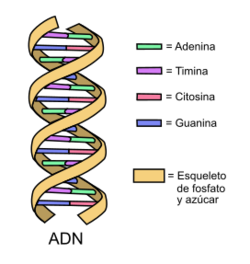
\includegraphics[width=0.4\linewidth]{DNA_simple2-es.png}
    %     \end{figure}
    % \end{frame}

    % \begin{frame}{String y ADN}
    %     \begin{tabular}{| p{4cm}| p{6cm}|}
    %     \hline
    %     \textbf{En strings} & \textbf{En ADN} \\ \hline
    %     Caracteres del alfabeto & Las 4 bases: A, T, G, C \\ \hline
    %     Longitud \mintinline{python}{len()} & Número de bases en la cadena \\ \hline
    %     Posición \mintinline{python}{x[i]} & Ubicación de una base específica \\ \hline
    %     Fragmento \mintinline{python}{x[a:b]} & Segmento o gen extraído \\ \hline
    %     \mintinline{python}{replace()} & Mutación: una base cambia por otra \\ \hline
    %     \mintinline{python}{count()} & Frecuencia de una base en la cadena \\ \hline
    %     \mintinline{python}{find()} & Localizar una secuencia en el genoma \\ \hline
    %     \end{tabular}
        
    %     \textbf{El ADN es el string más importante de la naturaleza}
    % \end{frame}

    \begin{frame}[fragile,t]{Propiedad del string}
        Un string \textbf{no se puede modificar una vez creado}
        \begin{minted}[xleftmargin=-2cm, frame=leftline, fontsize=\small]{python}
            s = "hola"
            s.upper()       # esto NO modifica s
            print(s)        # sigue siendo "hola"
            
            s = s.upper()   # SI modifica s, crea uno nuevo y lo reasigna
            print(s)        # ahora es "HOLA"
        \end{minted}
    \end{frame}

    \begin{frame}[fragile, t]{Concatenación y repetición}
        \begin{itemize}
            \item Concatenación
            \begin{minted}[xleftmargin=-2cm, frame=leftline, fontsize=\small]{python}
            nombre1 = "Universidad"
            nombre2 = "Catolica"

            completo = nombre1 + " " + nombre2   # "Universidad Catolica"
            \end{minted}
            \item Repetición
            \begin{minted}[xleftmargin=-2cm, frame=leftline, fontsize=\small]{python}
            separador = "-" * 20              # "--------------------"
            \end{minted}
        \end{itemize}
    \end{frame}

    \begin{frame}[fragile, t]{Strings y variables: f-strings}
        Construir texto dinámico
        \begin{minted}[xleftmargin=-2cm, frame=leftline, fontsize=\small]{python}
            nombre = "Pedro"
            edad = 40
            ciudad = "Santiago"
            
            # Forma antigua (incómoda)
            mensaje = "Hola, me llamo " + nombre + " y tengo " + \
                    str(edad) + " años."
            
            # f-string (forma moderna, mucho más clara)
            mensaje = f"Hola, me llamo {nombre} y tengo {edad} años."
            print(mensaje)   # "Hola, me llamo Pedro y tengo 40 años."
            
            # Incluso puedes poner expresiones dentro
            print(f"El doble de tu edad es {edad * 2}")
        \end{minted}
    \end{frame}

    \begin{frame}[fragile, t]{Conversión entre strings y otros tipos}
        Los strings son la forma en que los datos "entran" y "salen" de tu programa:
        \begin{minted}[xleftmargin=-2cm, frame=leftline, fontsize=\small]{python}
            # El usuario siempre ingresa texto, aunque escriba un número
            edad_texto = input("¿Cuántos años tienes? ")
            edad_numero = int(edad_texto)                
            
            # Para mostrar números como texto
            precio = 9990
            print("El precio es $" + str(precio))   
            print(f"El precio es ${precio}")        
        \end{minted}
    \end{frame}

    \begin{frame}[fragile, t]{Recorrer un string con \mintinline{python}{for} y \mintinline{python}{while}}
        Acceder a cada letra de un string con \mintinline{python}{for}
        \begin{minted}[xleftmargin=-2cm, frame=leftline, fontsize=\small]{python}
            palabra = "hola"
            for indice in range(len(palabra)):
                letra = palabra[indice]
                print(letra, indice)
        \end{minted}
        Acceder a cada letra de un string con \mintinline{python}{while}
        \begin{minted}[xleftmargin=-2cm, frame=leftline, fontsize=\small]{python}
            palabra = "hola"
            indice = 0
            while indice < len(palabra):
                letra = palabra[indice]
                print(letra, indice)
                indice += 1
        \end{minted}
    \end{frame}

    \begin{frame}[fragile, t]{Recorrer un string con \mintinline{python}{for}}
        Imprimir cada letra de un string
        \begin{minted}[xleftmargin=-2cm, frame=leftline, fontsize=\small]{python}
            palabra = "hola"
            for letra in palabra:
                print(letra)
        \end{minted}
        Contar las vocales en un string
        \begin{minted}[xleftmargin=-2cm, frame=leftline, fontsize=\small]{python}
            n_vocales = 0
            for letra in "Universidad Catolica":
                if letra.lower() in "aeiou":
                    n_vocales += 1
            print(n_vocales)   # 9
        \end{minted}
    \end{frame}

    \begin{frame}[fragile, t]{Recorrer un string con \mintinline{python}{while}}
        Contar las vocales en un string
        \begin{minted}[xleftmargin=-2cm, frame=leftline, fontsize=\small]{python}
            n_vocales = 0
            indice = 0
            palabra = "Universidad Catolica"
            while indice < len(palabra):
                letra = palabra[indice]
                if letra.lower() in "aeiou":
                    n_vocales += 1
                indice += 1
            print(n_vocales)   # 9
        \end{minted}
    \end{frame}
\end{document}
